\documentclass[12pt, a4paper]{article}

\usepackage[hmargin=2.5cm, vmargin=2cm]{geometry}
\usepackage{amsthm, amssymb, mathtools, yhmath, graphicx}
\usepackage{fontspec, type1cm, titlesec, titling, fancyhdr, tabularx}
\usepackage{color}
\usepackage{unicode-math}
\usepackage{float}
\usepackage{hhline}

\usepackage[CheckSingle, CJKmath]{xeCJK}
\usepackage{CJKulem}
\usepackage{enumitem}
%\setmainfont{Cantarell}
\setmonofont{Consolas}
\setCJKmainfont[BoldFont=cwTeX Q Hei]{cwTeX Q Ming}

\def\normalsize{\fontsize{12}{18}\selectfont}
\def\large{\fontsize{14}{21}\selectfont}
\def\Large{\fontsize{16}{24}\selectfont}
\def\LARGE{\fontsize{18}{27}\selectfont}
\def\Huge{\fontsize{20}{30}\selectfont}

\titleformat{\section}{\bf\Large}{\arabic{section}}{24pt}{}
\titleformat{\subsection}{\large}{\arabic{subsection}.}{12pt}{}
\titlespacing*{\subsection}{0pt}{0pt}{1.5ex}

\parindent=24pt

\DeclarePairedDelimiter{\abs}{\lvert}{\rvert}
\DeclarePairedDelimiter{\norm}{\lVert}{\rVert}
\DeclarePairedDelimiter{\inpd}{\langle}{\rangle}
\DeclarePairedDelimiter{\ceil}{\lceil}{\rceil}
\DeclarePairedDelimiter{\floor}{\lfloor}{\rfloor}

\newcommand{\unit}[1]{\:(\text{#1})}

\title{ \bf {\Huge 電子電路實驗一:Pspice 電路模擬}\\ 實驗結報}
\author{B02901178 江誠敏}
\date{2014/09/21} 

\begin{document}

\maketitle

\section{預報問題}
\begin{enumerate}[itemsep=20pt, topsep=10pt]
	\item {\large 目前OrCAD下載網頁最新版的OrCAD Demo Version是第幾版?} \\[10pt]
		答: 16.6 \footnote{http://www.orcad.com/resources/orcad-downloads}
\end{enumerate}

\section{實驗結果}

\subsection{工作點分析}

\begin{figure}[H]
	\begin{center}
		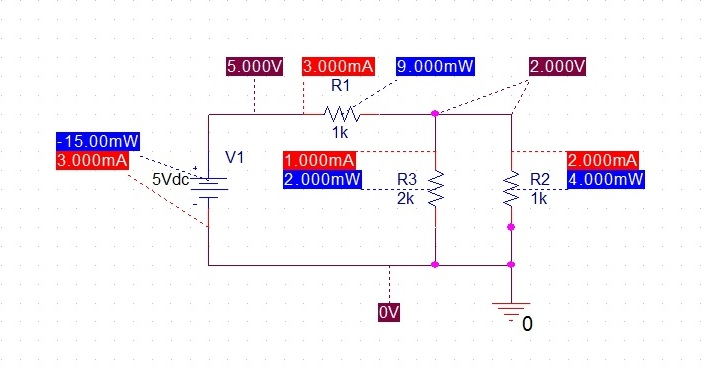
\includegraphics[width=10cm]{data/q1.jpg}
		\caption{實驗一模擬結果}
		\label{fig:fig1}
	\end{center}
\end{figure}

由Figure \ref{fig:fig1}可以得到:\\
\begin{center}
\begin{tabular}{|p{4cm}|p{4cm}|p{4cm}|}
	\hline
	電阻 & 端電壓 & 電流 \\
	\hhline{|=|=|=|}
	R1 & $3.0 \unit{V}$ & $3.0 \unit{mA}$ \\
	\hline
	R2 & $2.0 \unit{V}$ & $2.0 \unit{mA}$ \\
	\hline
	R3 & $2.0 \unit{V}$ & $1.0 \unit{mA}$ \\
	\hline
\end{tabular}
\end{center}

\clearpage

\subsection{直流分析}

\begin{figure}[H]
	\begin{center}
		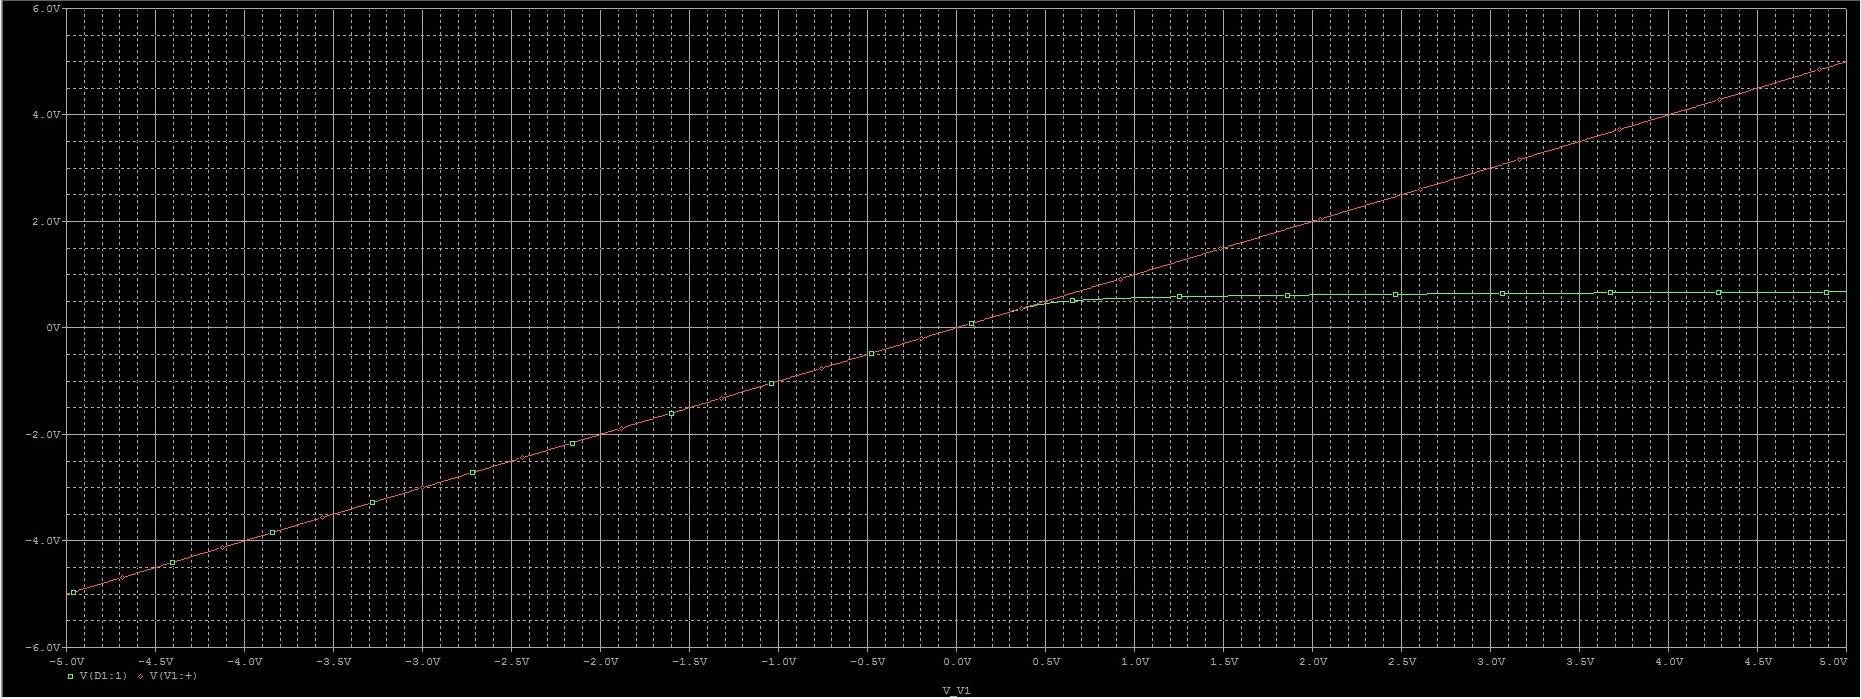
\includegraphics[width=15cm]{data/q2.jpg}
		\caption{實驗二模擬結果}
		\label{fig:fig2}
	\end{center}
\end{figure}

將Pspice的資料輸出後重新畫出一個較清析的圖如下:
\begin{figure}[H]
	\begin{center}
		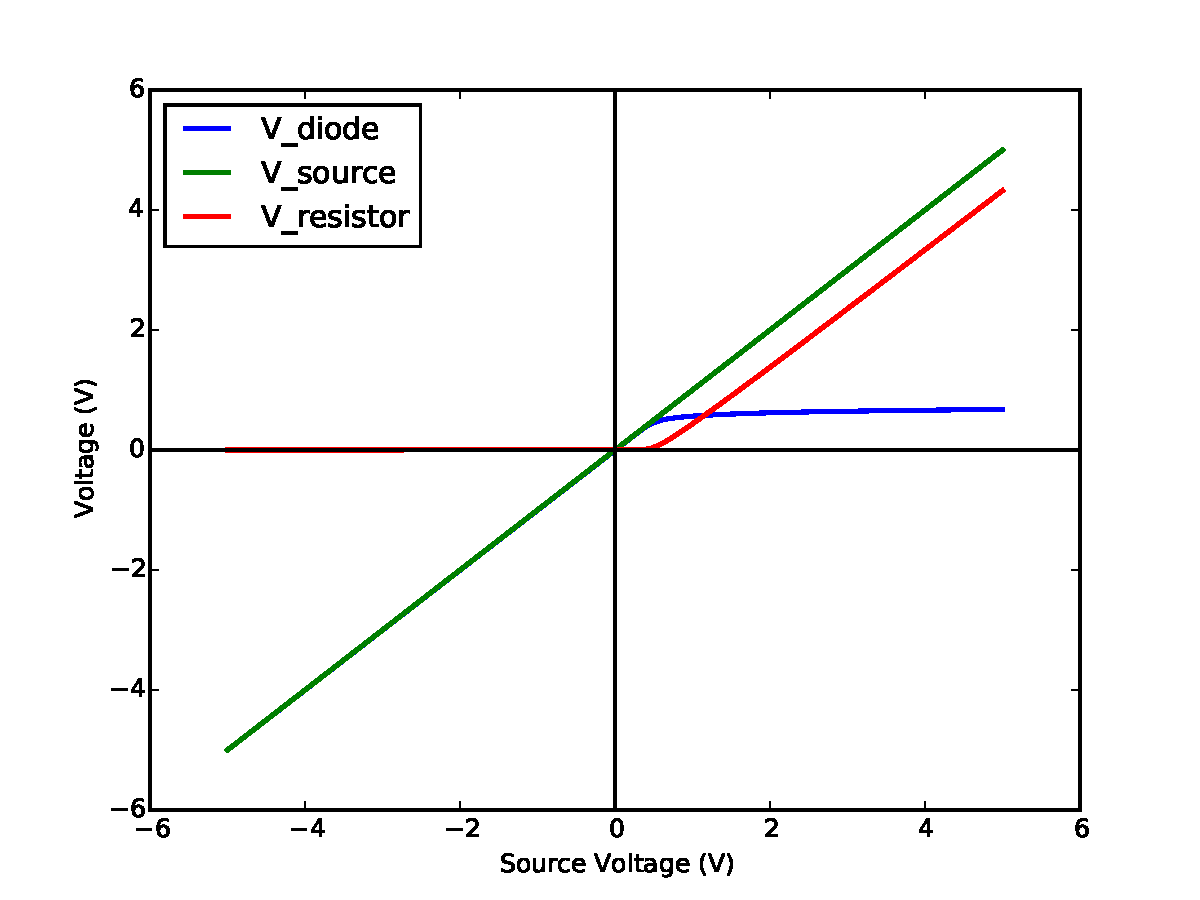
\includegraphics[width=10cm]{data/q2i.pdf}
		\caption{實驗二模擬結果}
		\label{fig:fig2-1}
	\end{center}
\end{figure}
可以在圖中看出二極體的性質,在一定電壓下是不導通的。

\subsection{暫態分析}

\begin{figure}[H]
	\begin{center}
		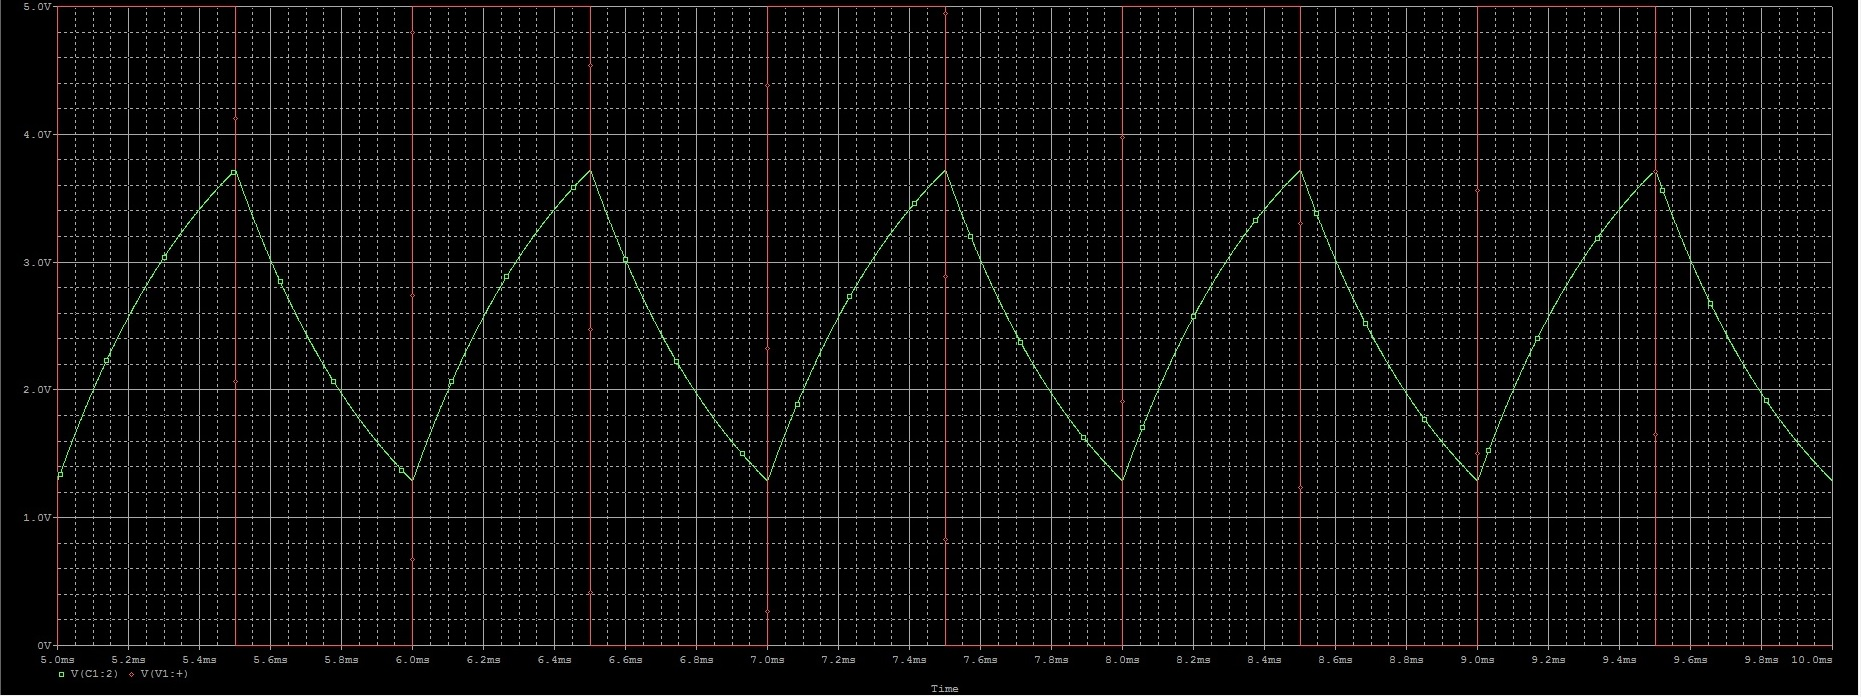
\includegraphics[width=15cm]{data/q3.jpg}
		\caption{實驗三模擬結果}
		\label{fig:fig3}
	\end{center}
\end{figure}

\begin{figure}[H]
	\begin{center}
		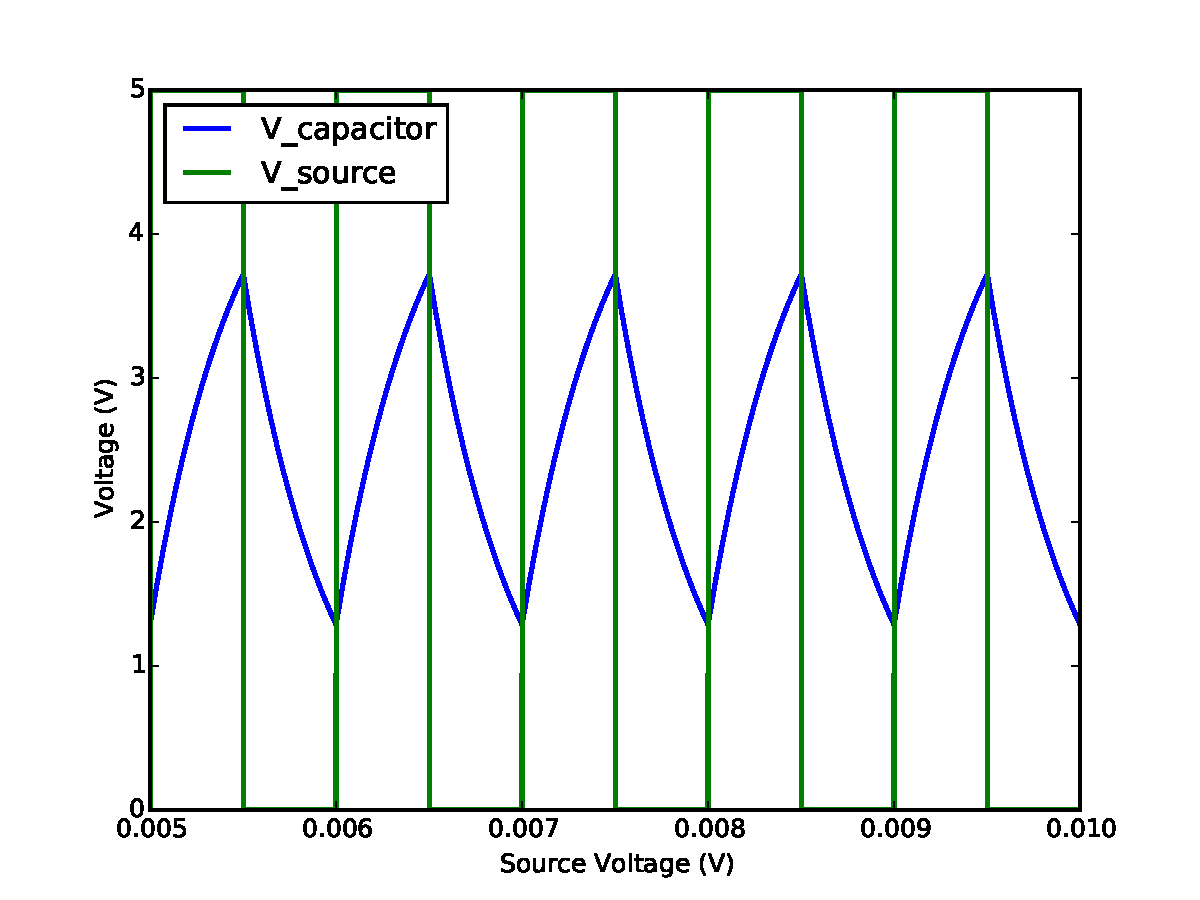
\includegraphics[width=10cm]{data/q3i.pdf}
		\caption{實驗三模擬結果}
		\label{fig:fig3}
	\end{center}
\end{figure}
可以看到電容充放電的情形。

\subsection{交流分析}

\begin{figure}[H]
	\begin{center}
		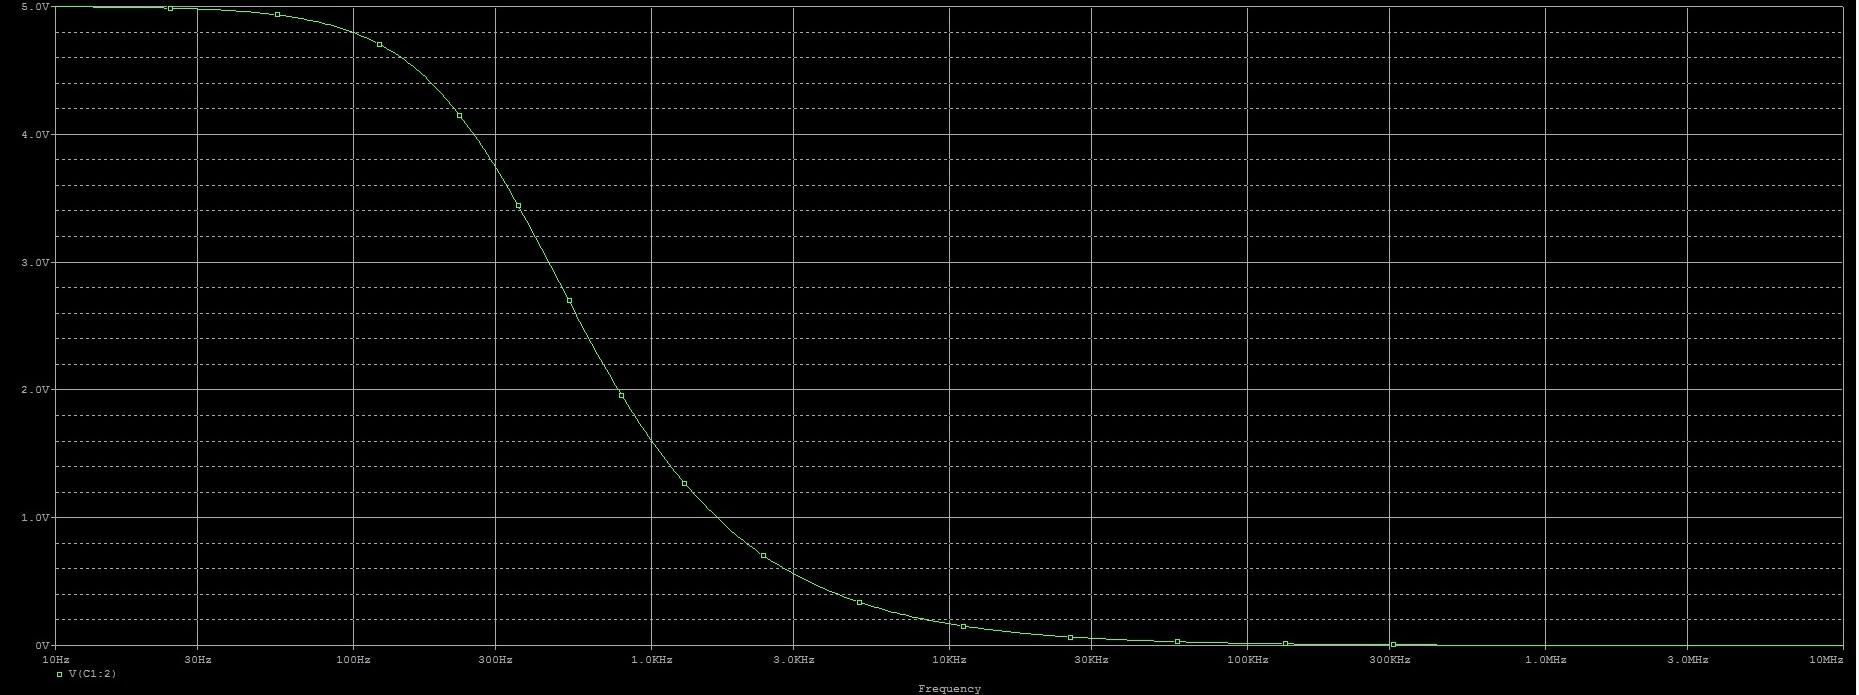
\includegraphics[width=15cm]{data/q4.jpg}
		\caption{實驗四模擬結果}
		\label{fig:fig4}
	\end{center}
\end{figure}

\begin{figure}[H]
	\begin{center}
		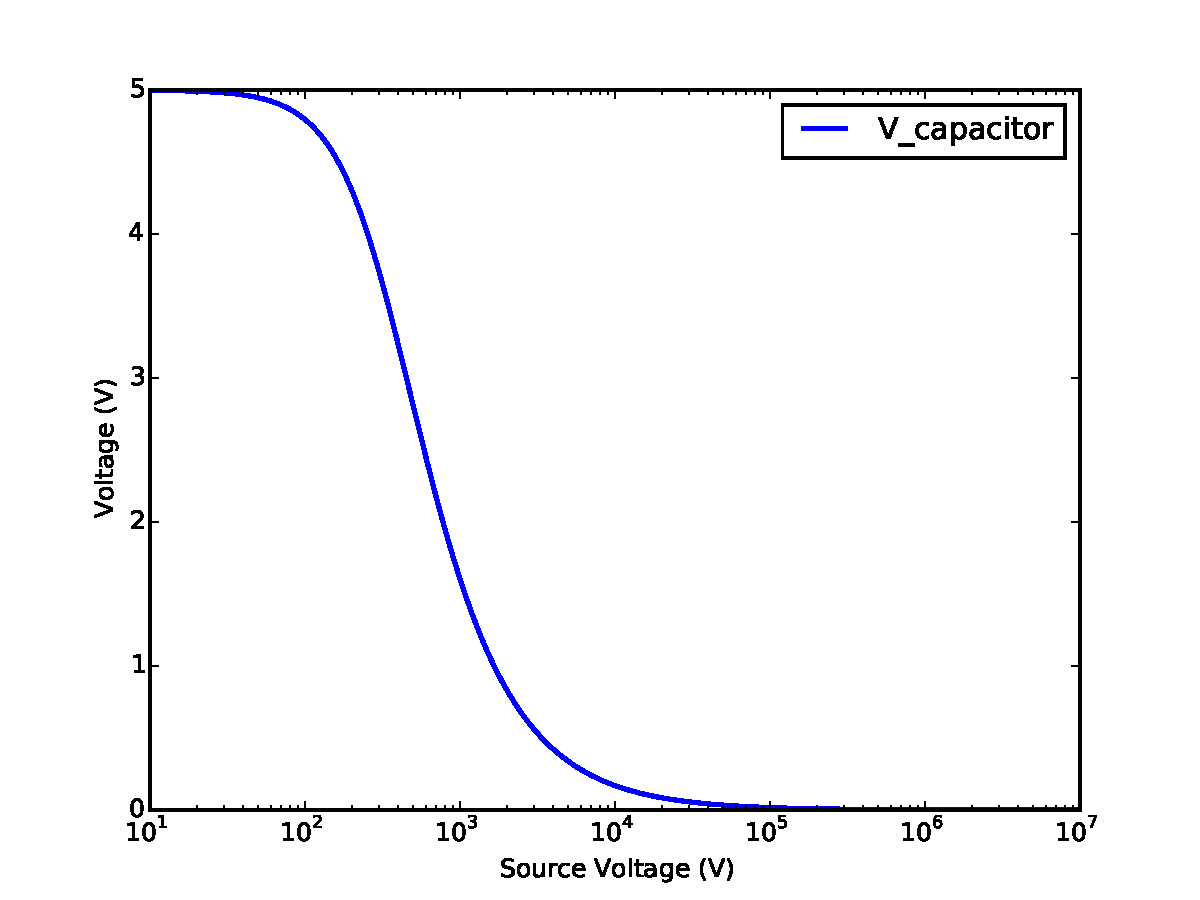
\includegraphics[width=10cm]{data/q4i.pdf}
		\caption{實驗四模擬結果}
		\label{fig:fig4}
	\end{center}
\end{figure}
可以看出此電路讓低頻信號通過。


\section{結報問題}

\begin{enumerate}[itemsep=20pt, topsep=10pt]
	\item {\large 有關於PSpice模擬分析的四種模式,用途分別為何?試說明之。} \\[10pt]
		答:PSpice的模擬分析有以下四種模式:
		\begin{enumerate}[itemsep=0ex, topsep=0ex, label=(\arabic*)]
			\item Bias Point : 計算在直流穩定態時,各個元件的端電壓、電流與功率。
			\item DC Sweep:模擬直流電源的電壓在不同值時,各個元件的反應、端電壓等等。
			\item Time Domain (Traisient):模擬交流電路,電路屬性對時間的變化。
			\item AC Sweep:模擬交流電路在不同頻率下的反應。
		\end{enumerate}

	\item {\large 電路模擬除了PSpice之外,另外還有其他哪些軟體可以使用?請盡量列舉。}\\[10pt]
		答:以下列舉出一些電路模擬程式
		\begin{enumerate}[itemsep=0ex, topsep=0ex, label=(\arabic*)]
			\item LTSpice:免費且開源的電路模擬程式,不會受到如Pspice Demo版節點數等限制。可以在Windows和OS X下運行。
			\item Qucs:Linux底下模擬電路的程式,免費小巧但功能較少。
			\item NGSpice:Linux下文字介面的電路模擬程式,特色是不用圖形介面,電路的描述等全用文字檔完成。
		\end{enumerate}
		其它還有HSpice, IS-Spice等等,這些程式大部分源自一個電路模擬程式- Spice。

\end{enumerate}


\end{document}

